% main.tex — Paper 3: How Language Models Organize Competing Moral Frameworks.
% arXiv-targeted; NeurIPS 2025 preprint style.
%
% Build:
%   make pdf   — runs pandoc on each sections/<NN>.md, then latexmk
%   make clean — removes intermediate latex files
%
% Section files live in build/sections/<NN>.tex (generated from
% ../sections/<NN>.md by `make sections`).

\documentclass{article}

% --- NeurIPS 2025 style (preprint mode for arXiv) -------------------
\PassOptionsToPackage{round, comma, sort&compress, authoryear}{natbib}
\usepackage[preprint]{neurips_2025}
\bibliographystyle{plainnat}

% --- Typography -----------------------------------------------------
\usepackage[T1]{fontenc}
\usepackage[utf8]{inputenc}
\usepackage{microtype}
\usepackage{textcomp}
\setlength{\emergencystretch}{3em}

\PassOptionsToPackage{hyphens}{url}
\usepackage{url}
\urlstyle{tt}
\Urlmuskip=0mu plus 1mu

% --- Math ------------------------------------------------------------
\usepackage{amsmath}
\usepackage{amssymb}

% --- Tables -----------------------------------------------------------
\usepackage{booktabs}
\usepackage{array}
\usepackage{longtable}
\usepackage{calc}
\providecommand{\real}[1]{#1}
\setlength{\tabcolsep}{4pt}
\renewcommand{\arraystretch}{1.05}

% --- Lists ------------------------------------------------------------
\usepackage{enumitem}

% --- Captions ---------------------------------------------------------
\usepackage[font=small,labelfont=bf]{caption}

% --- Figures ----------------------------------------------------------
\usepackage{graphicx}
\graphicspath{{../figures/}{../outputs/figures/}}

% --- Color ------------------------------------------------------------
\usepackage{xcolor}

% --- Cross-references -------------------------------------------------
\usepackage[colorlinks=true,
            linkcolor=blue!50!black,
            citecolor=blue!50!black,
            urlcolor=blue!50!black]{hyperref}
\usepackage[capitalize, noabbrev]{cleveref}

% --- Title / authors --------------------------------------------------
\title{How Language Models Organize Competing Moral Frameworks}

\author{%
  Orion Reblitz-Richardson\thanks{%
    Distiller Labs. Correspondence to Distiller Labs
    \textless\texttt{orion@orionr.com}\textgreater.}
}

\date{May 2026}

% --- Pandoc stubs -----------------------------------------------------
\providecommand{\tightlist}{%
  \setlength{\itemsep}{0pt}\setlength{\parskip}{0pt}}

\newcounter{none}

\usepackage{fancyvrb}
\DefineVerbatimEnvironment{Highlighting}{Verbatim}{commandchars=\\\{\}}
\newenvironment{Shaded}{\begin{quote}}{\end{quote}}
\newcommand{\KeywordTok}[1]{\textbf{#1}}
\newcommand{\DataTypeTok}[1]{\textbf{#1}}
\newcommand{\StringTok}[1]{\textit{#1}}
\newcommand{\CommentTok}[1]{\textit{#1}}
\newcommand{\OperatorTok}[1]{#1}
\newcommand{\NormalTok}[1]{#1}
\newcommand{\BuiltInTok}[1]{#1}
\newcommand{\ExtensionTok}[1]{#1}
\newcommand{\ControlFlowTok}[1]{\textbf{#1}}
\newcommand{\FunctionTok}[1]{#1}
\newcommand{\VariableTok}[1]{#1}
\newcommand{\AttributeTok}[1]{#1}
\newcommand{\OtherTok}[1]{#1}
\newcommand{\PreprocessorTok}[1]{#1}
\newcommand{\DocumentationTok}[1]{\textit{#1}}
\newcommand{\InformationTok}[1]{\textit{#1}}
\newcommand{\ImportTok}[1]{\textbf{#1}}
\newcommand{\ConstantTok}[1]{#1}
\newcommand{\CharTok}[1]{\textit{#1}}
\newcommand{\SpecialCharTok}[1]{#1}
\newcommand{\VerbatimStringTok}[1]{\texttt{#1}}
\newcommand{\SpecialStringTok}[1]{\texttt{#1}}
\newcommand{\DecValTok}[1]{#1}
\newcommand{\BaseNTok}[1]{#1}
\newcommand{\FloatTok}[1]{#1}
\newcommand{\AlertTok}[1]{\textbf{#1}}
\newcommand{\ErrorTok}[1]{\textbf{#1}}
\newcommand{\WarningTok}[1]{#1}
\newcommand{\AnnotationTok}[1]{#1}
\newcommand{\CommentVarTok}[1]{\textit{#1}}
\newcommand{\RegionMarkerTok}[1]{#1}

% =====================================================================
\begin{document}

\maketitle

\begin{abstract}
How do language models organize moral knowledge? Models detect moral
content broadly, but detection is a low bar. We ask whether they go
further: distinguishing moral foundations from one another and
organizing the relationships between them.

Training six independent linear probes on OLMo-2~1B and 7B and
OLMoE-1B-7B, one per foundation in Moral Foundations Theory (MFT),
shows integration. Foundation directions in representation space are
geometrically distinct, spanning five effective dimensions, yet share
a common component, shown by a uniformly positive mean pairwise cosine
(the effective dimensionality rules out collapse but, at its ceiling
for six mean-centered directions, does not mark integration; the
positive cosine is what marks integration rather than isolation). That
positive cosine (0.26) is ${\sim}20\times$ a matched non-moral concept
battery built identically to the foundations (0.013; paired
$\Delta = 0.223$, CI [0.202, 0.244], excluding 0; all six non-moral
probes decode at 1.00), so the shared component is moral-specific
relative to a matched non-moral battery, not a generic
content-vs-neutral axis; whether it is specifically moral rather than
generic affective salience is the open residual. This
is genuine multi-dimensional structure, not a single moral detector. The geometry is consistent
across scale (1B to 7B dense), across dense and MoE architectures, and
on the independently constructed Moral Foundations Vignettes; across
pre-training it reaches this integration regime early (within a few
thousand steps, well before probing accuracy saturates) and then
slowly differentiates.

The structure the model develops shows no evidence of the
individualizing/binding distinction central to MFT: neither
hierarchical clustering of the probe directions nor unsupervised
clustering of the activations recovers it. The group-structure test is
underpowered (only 20 partitions, smallest achievable $p = 0.05$), so a
small effect is not excluded; we report no evidence of MFT grouping
rather than its absence. What structure the model does form is grounded
in corpus statistics rather than human theoretical categories. Seed-averaged fragility testing shows that output dilution
is foundation-uniform: every foundation is more fragile in MoE than in
dense, with no foundation reliably most or least robust within an
architecture.

Extending to moral dilemmas shows partial compositionality: each
dilemma direction projects only ${\sim}12$\% of its variance onto its
two component foundations (about $2.7\times$ a mismatched-pair
baseline), and the remaining ${\sim}88$\% encodes conflict-specific
structure beyond them, with balanced loading suggesting the model
represents moral conflict itself rather than a pre-resolved judgment.
\end{abstract}

% =====================================================================
\section{Introduction}\label{introduction}

How do language models represent morality? Prior work in this
series established that models encode moral content \emph{broadly}:
probing accuracy saturates early during pre-training and spans
nearly all layers \citep{reblitzrichardson2026fragility}. Fragility
testing revealed that this encoding grows more robust throughout
training even after accuracy plateaus. Extension to
mixture-of-experts (MoE) models showed that moral signal is
uniform across experts, with no expert specialization, but that a
77\(\times\) output scale gap produces structural fragility
\citep{reblitzrichardson2026dilution}.

Both papers treated moral encoding as a single binary feature:
moral vs.~neutral. A model that merely detects ``this text involves
morality'' has cleared a low bar. Genuine moral understanding
requires \emph{structured} representations --- the ability to distinguish
care from fairness, loyalty from authority, and to encode the
relationships between them. The transition from moral \emph{detection}
to moral \emph{understanding} is the subject of this paper.

We operationalize this transition through the geometry of
foundation-specific probe directions. Where prior work trained one
probe to separate moral from neutral content, we train six: one for
each Moral Foundations Theory (MFT) foundation
\citep{haidt2012righteous, graham2013mft}. The learned probe weight
vectors define \emph{directions} in the model's representation space.
The angular relationships between these directions reveal whether
the model has developed structured moral representations.

Three geometric signatures correspond to three qualitatively
different modes of moral representation:

\begin{enumerate}
\def\labelenumi{\arabic{enumi}.}
\item
  \textbf{Collapse.} All foundation directions converge toward a single
  ``moral salience'' direction. The model detects moral relevance
  but does not distinguish frameworks. This is detection without
  structure.
\item
  \textbf{Isolation.} Foundation directions are orthogonal with no
  relational structure. The model has separate moral ``slots'' but
  no representation of how frameworks relate. This is structure
  without coherence.
\item
  \textbf{Integration.} Foundation directions are separated but
  non-orthogonal, with inter-framework geometry reflecting known
  relationships from moral psychology. This is the precondition
  for moral reasoning.
\end{enumerate}

Applied to OLMo-2 1B and OLMoE-1B-7B, we find clear \emph{integration}:
foundation directions are distinct (mean pairwise cosine similarity
\(\approx 0.3\), far from collapse), and hierarchical clustering
recovers the MFT distinction between individualizing foundations
(care, fairness, liberty) and binding foundations (loyalty,
authority, sanctity). This alignment with theoretical predictions
from moral psychology emerges without explicit training signal ---
the model absorbs inter-framework structure from the distributional
statistics of the training corpus.

Extending the fragility protocol to per-foundation probes reveals a
cross-architectural reversal: in dense models, binding foundations
are the most robust; in MoE models, individualizing foundations are
more robust. The output dilution effect preferentially degrades
binding-foundation representations, suggesting that group-oriented
moral concepts are encoded through mechanisms that are more
vulnerable to the MoE routing structure.

This paper makes three contributions:

\begin{enumerate}
\def\labelenumi{\arabic{enumi}.}
\item
  \textbf{Framework-specific probing methodology.} We introduce probe
  direction geometry as a tool for measuring structured moral
  representations, bridging the gap between binary moral probing
  and the richer structure posited by moral psychology.
\item
  \textbf{Empirical geometric characterization.} We show that OLMo-2
  1B and OLMoE-1B-7B exhibit the integration signature, that
  inter-framework geometry reflects MFT predictions, and that
  framework geometry is comparable across the two architectures
  tested (dense vs.~MoE).
\item
  \textbf{Differential fragility.} We demonstrate that moral foundations
  differ in robustness, and that MoE architecture
  disproportionately degrades binding foundations --- the first
  evidence that output dilution is not foundation-uniform.
\end{enumerate}

\section{Related Work}\label{related-work}

\subsection{Probing for linguistic and semantic structure}\label{probing-for-linguistic-and-semantic-structure}

Linear probing \citep{alain2017probes} has become a standard tool
for reading off what information is encoded in neural network
representations. \citet{conneau2018probing} probed sentence
embeddings for syntactic properties; subsequent work probed for
part-of-speech, dependency relations, coreference, and world
knowledge. The linear representation hypothesis
\citep{park2024linear} formalizes the claim that concepts are
encoded as directions in representation space --- precisely the
assumption underlying our use of probe weight vectors as geometric
objects.

Two limitations of the probing literature motivate our approach.
First, most probing studies report only \emph{accuracy}, discarding the
learned probe parameters. We show that the probe weight vector ---
the normal to the classification hyperplane --- carries geometric
information about how concepts relate to each other. Second,
probing studies typically train one probe per concept, treating
concepts as independent. Our multi-probe geometric analysis
recovers inter-concept structure from independently trained probes.

\subsection{Geometry of concept representations}\label{geometry-of-concept-representations}

\citet{bolukbasi2016gender} demonstrated that gender bias in word
embeddings manifests as a geometric subspace, and that debiasing
amounts to projecting out a direction. \citet{arditi2024refusal}
showed that refusal behavior in instruction-tuned LLMs is mediated
by a single direction in activation space. These results establish
the precedent that high-level behavioral properties can be localized
to specific directions.

Our work extends this line from single directions to \emph{sets of
related directions}. Where prior work asked ``where is concept \(X\)?''
we ask ``what is the geometric relationship between concepts
\(X_1, \ldots, X_k\)?'' The cosine similarity matrix between
foundation probe directions is a form of representational similarity
analysis \citep[RSA;][]{kriegeskorte2008rsa} applied not to stimulus
response patterns but to the probes that decode them.

\subsection{Moral psychology and Moral Foundations Theory}\label{moral-psychology-and-moral-foundations-theory}

Moral Foundations Theory \citep[MFT;][]{haidt2012righteous,
graham2013mft} posits that human moral judgment draws on (at least)
five or six innate foundations: care/harm, fairness/cheating,
loyalty/betrayal, authority/subversion, sanctity/degradation, and
(later added) liberty/oppression. MFT predicts a structural
distinction between \emph{individualizing} foundations (care, fairness,
liberty), which protect individuals from harm, and \emph{binding}
foundations (loyalty, authority, sanctity), which bind individuals
into groups. This distinction has been validated in cross-cultural
surveys and predicts political orientation
\citep{graham2013mft}.

Alternative taxonomies exist. \citet{curry2019cooperation} propose
morality-as-cooperation, identifying seven moral domains grounded
in evolutionary game theory. Our use of MFT is pragmatic: the
six-foundation taxonomy provides a tractable set of directions for
geometric analysis, and the individualizing/binding prediction
provides a testable structural hypothesis.

\subsection{Moral reasoning in language models}\label{moral-reasoning-in-language-models}

\citet{hendrycks2021ethics} introduced the ETHICS benchmark for
evaluating moral reasoning in language models across justice,
deontology, virtue, utilitarianism, and commonsense dimensions.
Most work in this area evaluates models \emph{behaviorally} ---
measuring what outputs models produce in response to moral
scenarios. Our approach is \emph{representational}: we probe the
internal geometry of moral encoding, asking not whether the model
produces the right moral judgment but whether it has developed
structured representations of moral distinctions.

\subsection{Companion papers}\label{companion-papers}

This paper is the third in a series. Paper 1
\citep{reblitzrichardson2026fragility} established that moral
content is decodable by linear probes from the earliest layer
of OLMo-2, that probing accuracy saturates early during
pre-training, and that fragility testing --- injecting Gaussian
noise into activations --- resolves the continued development of
moral encoding after accuracy plateaus. Paper 2
\citep{reblitzrichardson2026dilution} extended the analysis to
MoE models (OLMoE-1B-7B), finding uniform moral encoding across
experts but a 74\(\times\) output scale gap that produces structural
fragility.

The present paper moves from \emph{binary} moral encoding (moral
vs.~neutral) to \emph{structured} moral encoding (framework-specific
directions and their inter-framework geometry). It reuses the
probing and fragility protocols from Papers 1 and 2, applying
them at the per-foundation level.

\section{Methodology}\label{methodology}

We train six foundation-specific linear probes at each transformer
layer, extract the learned weight vectors as geometric directions in
representation space, and analyze the angular relationships between
these directions. The methodology decomposes into five components:
foundation-specific probing (\Cref{foundation-specific-probing}), geometric analysis of probe
directions (\Cref{geometric-analysis}), bootstrap direction stability assessment (\Cref{bootstrap-direction-stability}),
framework-specific fragility testing (\Cref{framework-specific-fragility}), and the probing
dataset (\Cref{probing-dataset}). All experiments run on a single MacBook Pro M4 Pro
(24 GB unified memory, MPS backend).

\subsection{Models and comparison design}\label{models-and-comparison-design}

We evaluate three base (non-instruct) models from the same lab
(Ai2). The primary comparison is between two architectures matched in
layer count (16), dense vs.~mixture-of-experts; a third, larger dense
model serves as a scale control (\S4.14):

\begin{itemize}
\item
  \textbf{OLMo-2 1B} (\path|allenai/OLMo-2-0425-1B|): dense transformer,
  1.5B parameters, 2048 hidden dimension, 16 layers \citep{olmo2_2025}.
  Ai2 publishes 37 early-training checkpoints at 1K-step intervals
  (steps 0--36K), enabling trajectory analysis.
\item
  \textbf{OLMoE-1B-7B} (\path|allenai/OLMoE-1B-7B-0924|): mixture-of-experts,
  6.9B total parameters, 1.3B active, 64 experts per layer, top-8
  routing, 2048 hidden dimension, 16 layers \citep{muennighoff2024olmoe}.
\item
  \textbf{OLMo-2 7B} (\path|allenai/OLMo-2-1124-7B|): dense transformer, 7.3B
  parameters, 4096 hidden dimension, 32 layers \citep{olmo2_2025}. Used
  in \S4.14 to test whether the geometry findings persist with scale.
\end{itemize}

All three models use the same tokenizer and comparable training corpora.
The comparison tests whether framework geometry is an artifact of
dense connectivity or a general property of transformer-based
language modeling. \citet{reblitzrichardson2026dilution} established
that moral encoding in OLMoE is uniform across experts with a
74\(\times\) output scale gap relative to OLMo-2; the present work
asks whether this output dilution affects the \emph{structure} of moral
representations, not just their \emph{scale}.

\subsection{Foundation-specific probing}\label{foundation-specific-probing}

For each of the six Moral Foundations Theory (MFT) foundations
(care/harm, fairness/cheating, loyalty/betrayal, authority/subversion,
sanctity/degradation, and liberty/oppression;
\citep{haidt2012righteous, graham2013mft}), we train a binary
linear probe at each of 16 transformer layers.

\textbf{Probe architecture.} Each probe is \texttt{nn.Linear(2048,\ 1)} trained
with BCE loss and Adam (lr = \(10^{-2}\)) for 50 epochs. This
matches the probe specification from
\citet{reblitzrichardson2026fragility} and
\citet{reblitzrichardson2026dilution}, enabling direct comparison
with their binary moral/neutral probes.

\textbf{Activation collection.} For each text, we run a single forward
pass capturing all 16 layers simultaneously. At each layer, we
mean-pool across the sequence dimension to obtain a single
\(\mathbb{R}^{2048}\) vector per text. Positive examples are the
foundation-tagged moral sentences; negative examples are their
matched neutral counterparts.

\textbf{Direction extraction.} After training, we extract the weight
vector \(\mathbf{w} \in \mathbb{R}^{2048}\) from each probe and
normalize to unit length: \(\hat{\mathbf{w}} = \mathbf{w} /
\|\mathbf{w}\|\). This unit vector is the normal to the
classification hyperplane, the \emph{direction} in representation
space that maximally separates the foundation's moral content from
neutral content. We call \(\hat{\mathbf{w}}\) the foundation's
\textbf{probe direction} at a given layer.

This yields \(6 \times 16 = 96\) unit-norm probe direction vectors
per model.

\subsection{Geometric analysis}\label{geometric-analysis}

The paper's core contribution is analyzing the angular relationships
between the six foundation probe directions at each layer.

\textbf{Cosine similarity matrices.} At each layer, we compute the
\(6 \times 6\) pairwise cosine similarity matrix of the foundation
probe directions. Because the directions are unit-normalized,
\(\cos(\hat{\mathbf{w}}_i, \hat{\mathbf{w}}_j) =
\hat{\mathbf{w}}_i \cdot \hat{\mathbf{w}}_j\).

\textbf{Geometric signatures.} Three qualitative modes of moral
representation correspond to distinct cosine similarity patterns:

\begin{enumerate}
\def\labelenumi{\arabic{enumi}.}
\item
  \emph{Collapse (averaging).} All foundation directions converge
  toward a single ``moral salience'' direction. Mean pairwise
  cosine similarity \(\to 1\).
\item
  \emph{Isolation.} Foundation directions are orthogonal with no
  relational structure. Mean pairwise cosine similarity \(\to 0\).
\item
  \emph{Integration.} Foundation directions are separated but
  non-orthogonal, with inter-framework geometry reflecting known
  relationships. Mean pairwise cosine similarity in \((0, 1)\) with
  structured variation.
\end{enumerate}

\textbf{Effective dimensionality.} We compute the effective
dimensionality of the 6-direction set at each layer via PCA on
the \(6 \times 2048\) matrix of probe directions. Effective
dimensionality is the number of principal components explaining
\(\geq 90\%\) of variance. Low dimensionality (1--2) indicates
collapse; high dimensionality (5--6) indicates separation.

\textbf{Hierarchical clustering.} We apply Ward's method to the cosine
distance matrix (\(1 - \cos(\cdot, \cdot)\)) at each layer.
Dendrograms reveal whether the six foundations cluster into
interpretable groups.

\textbf{Permutation test for MFT group structure.} MFT predicts that
the six foundations divide into \emph{individualizing} (care, fairness,
liberty) and \emph{binding} (loyalty, authority, sanctity) clusters
\citep{graham2013mft}. We test this prediction with a permutation
test: compute the observed difference between mean within-group
cosine similarity and mean between-group cosine similarity, then
permute group assignments 10,000 times to generate the null
distribution.

\subsection{Bootstrap direction stability}\label{bootstrap-direction-stability}

With 32 training pairs per foundation in 2048 dimensions, the probe
has 2049 parameters and only 64 training examples. The classification
\emph{accuracy} may be robust in this regime (a single hyperplane suffices
for binary separation), but the extracted \emph{direction} could be noisy
, and noise in directions contaminates the angular analysis.

We assess direction stability via bootstrap resampling: for each
foundation at each layer, we resample the 32 training pairs with
replacement 200 times, retrain the probe on each bootstrap sample,
and compute the cosine similarity of each bootstrap direction with
the full-data direction. A mean bootstrap cosine similarity \(> 0.8\)
indicates a stable direction.

This gives a per-layer, per-foundation reliability metric for the
geometric analysis. Layers where directions are unstable should be
interpreted with caution.

\subsection{Framework-specific fragility}\label{framework-specific-fragility}

We extend the fragility protocol of
\citet{reblitzrichardson2026fragility} to per-foundation probes.
For each foundation at each layer:

\begin{enumerate}
\def\labelenumi{\arabic{enumi}.}
\tightlist
\item
  Train a linear probe on clean activations.
\item
  Evaluate on clean test activations (baseline accuracy).
\item
  For each noise level \(\sigma \in \{0.1, 0.3, 1.0, 3.0, 10.0\}\),
  add \(\mathcal{N}(0, \sigma^2)\) noise to cached test activations
  and re-evaluate.
\item
  The \textbf{critical noise} \(\sigma^*\) is the smallest \(\sigma\) where
  accuracy drops below 0.6.
\end{enumerate}

This tests the universality hypothesis: more cross-culturally
universal foundations (care/harm) should be more robustly encoded
than culturally variable foundations (sanctity/degradation,
loyalty/betrayal). Cross-architectural comparison tests whether
the output dilution effect \citep{reblitzrichardson2026dilution}
affects all foundations uniformly.

\subsection{Probing dataset}\label{probing-dataset}

We use the same 240-pair minimal-pair probing dataset from
\citet{reblitzrichardson2026fragility}, now used at the
per-foundation level: 40 pairs per MFT foundation, stratified
80/20 into 32 train and 8 test pairs per foundation. Each pair
consists of a moral sentence tagged with its MFT foundation and a
matched neutral sentence controlling for sentence length, syntactic
structure, and topic. The dataset was drawn from a 1\{,\}200-pair
candidate pool generated by Claude Sonnet 4.6 from hand-written
seed examples, with automated validation gates (length ratio \(\leq
1.5\), embedding similarity, keyword scan, deduplication) and
LLM-as-judge filtering for neutral-pair quality.

For the geometric analysis, the 32 training pairs per foundation
yield \(64\) training examples (moral + neutral) for the
\texttt{nn.Linear(2048,\ 1)} probe. While this is a small sample for a
2049-parameter model, the bootstrap stability analysis (\Cref{bootstrap-direction-stability})
directly quantifies whether the resulting directions are reliable.

\subsection{Dilemma compositionality analysis}\label{dilemma-compositionality-analysis}

Experiments 1--7 establish that the model maintains distinct
directions for each moral foundation. A natural follow-up: when
two foundations \emph{conflict} in a moral dilemma, does the model
represent the dilemma as a composition of its component foundation
directions, or does it develop a qualitatively new representation?

\textbf{Dilemma dataset.} We generate 300 moral dilemma scenarios (20
per each of the \(\binom{6}{2} = 15\) foundation pairs) using
Claude Sonnet 4.6, with hand-written seed examples per pair. Each
scenario pits two specific foundations against each other (e.g.,
care vs.~authority: ``The nurse administered an unapproved
painkiller to a dying patient because following protocol meant
hours more agony''). Each dilemma text is paired with a matched
neutral sentence. All pairs pass automated validation gates
(length ratio, keyword scan, deduplication).

\textbf{Dilemma-specific probes.} For each of the 15 foundation pairs,
we train a binary linear probe (same architecture as \Cref{foundation-specific-probing}) to
distinguish dilemma moral text from matched neutral text. The
probe weight vector \(\hat{\mathbf{w}}_{\text{dilemma}}\) is the
direction in representation space that separates the dilemma
content from neutral content.

\textbf{Subspace membership score.} To measure compositionality, we
project each dilemma direction onto the 2D subspace spanned by its
two component foundation directions. Given component directions
\(\hat{\mathbf{w}}_A\) and \(\hat{\mathbf{w}}_B\) from Experiment 1,
we orthogonalize them via Gram--Schmidt and compute the fraction
of the dilemma direction's variance explained by this 2D subspace:

\[S = \|\text{proj}_{\text{span}(\hat{\mathbf{w}}_A, \hat{\mathbf{w}}_B)} \hat{\mathbf{w}}_{\text{dilemma}}\|^2\]

A membership score of \(S = 1\) indicates full compositionality
(the dilemma direction lies entirely within the component
subspace); \(S = 0\) indicates complete independence. The null
baseline for a random unit vector in \(\mathbb{R}^{2048}\) projected
onto a random 2D subspace has expected membership \(2/2048 \approx
0.001\). We estimate the empirical null distribution from 10\{,\}000
random unit vectors.

\textbf{Component balance.} We decompose the within-subspace projection
into components along \(\hat{\mathbf{w}}_A\) and the
Gram--Schmidt-orthogonalized \(\hat{\mathbf{w}}_B\). The balance
ratio (fraction of the projection along the first component)
measures whether the dilemma direction is dominated by one
foundation or draws equally on both. A ratio near 0.5 indicates
balanced composition.

\textbf{Shared-component geometry.} If dilemma representations are
partially compositional, dilemma pairs that share a foundation
component should have more similar probe directions than pairs
with no shared foundation. We test this by comparing the mean
cosine similarity between dilemma directions for pairs that share
a component (e.g., care--fairness and care--loyalty, which share
care) versus pairs with no overlap (e.g., care--fairness and
loyalty--sanctity).

\textbf{Cross-architecture consistency.} We repeat the dilemma probing
and subspace analysis on OLMoE-1B-7B to test whether the
compositionality structure is architecture-specific or general.

\section{Results}\label{results}

\subsection{Foundation-specific probe accuracy}\label{foundation-specific-probe-accuracy}

All six foundation-specific probes achieve near-perfect accuracy
across the full depth of OLMo-2 1B. Care/harm and fairness/cheating
reach 100\% at nearly every layer; sanctity/degradation reaches
100\% at 12 of 16 layers. Liberty/oppression, loyalty/betrayal, and
authority/subversion show minor fluctuations (minimum 87.5\%, at
layers 3 and 15 for loyalty and layers 6 and 13--15 for authority).
The onset threshold (0.6) is exceeded at layer 0 for all
foundations.

These results confirm that moral foundation content is linearly
separable from the earliest layer --- consistent with the ``immediate
onset'' finding of \citet{reblitzrichardson2026fragility} for the
pooled binary moral/neutral probe. The per-foundation decomposition
reveals no qualitative difference in \emph{detectability} across
foundations: all are equally easy to decode. The interesting
variation is not in accuracy but in the \emph{geometry} of the probe
directions that achieve this accuracy.

On OLMoE-1B-7B, all foundations similarly reach near-perfect
accuracy, with authority/subversion showing the lowest peak (93.8\%
at layer 0). The accuracy profiles are essentially indistinguishable
between architectures.

\subsection{Framework geometry: integration, not collapse}\label{framework-geometry-integration-not-collapse}

\begin{figure}[t]
\centering

\includegraphics[width=\linewidth]{fig1_cosine_heatmap.pdf}
\caption{Pairwise cosine similarity between foundation probe directions at layer 0 (peak separation), OLMo-2 1B. Individualizing foundations (care, fairness, liberty) show higher within-group similarity than between-group pairs.}
\label{fig:cosine_heatmap}
\end{figure}

The headline finding: foundation probe directions are \emph{separated},
not collapsed. At the peak separation layer (layer 0), the mean
pairwise cosine similarity between the six foundation directions is
\textbf{0.272} --- far below the collapse threshold (\(>0.95\)) and below
the intermediate zone (\(0.8\)--\(0.95\)). The model does not encode
moral content through a single ``moral salience'' direction; it
maintains distinct directions for distinct moral foundations.

However, the cosine similarities are uniformly \emph{positive} (range
0.18--0.37 at layer 0), indicating that the foundation directions
share a common component. This is the \emph{integration} signature from
our trichotomy: the directions are separated but non-orthogonal,
consistent with a shared moral-salience subspace from which
foundation-specific directions deviate.

\textbf{Effective dimensionality.} The six foundation directions span
5 effective dimensions (the number of PCs explaining \(\geq 90\%\)
of variance) at every layer. This is near the maximum possible for
6 directions, confirming that the directions are geometrically
distinct --- they do not collapse into a lower-dimensional subspace.

\begin{figure}[t]
\centering
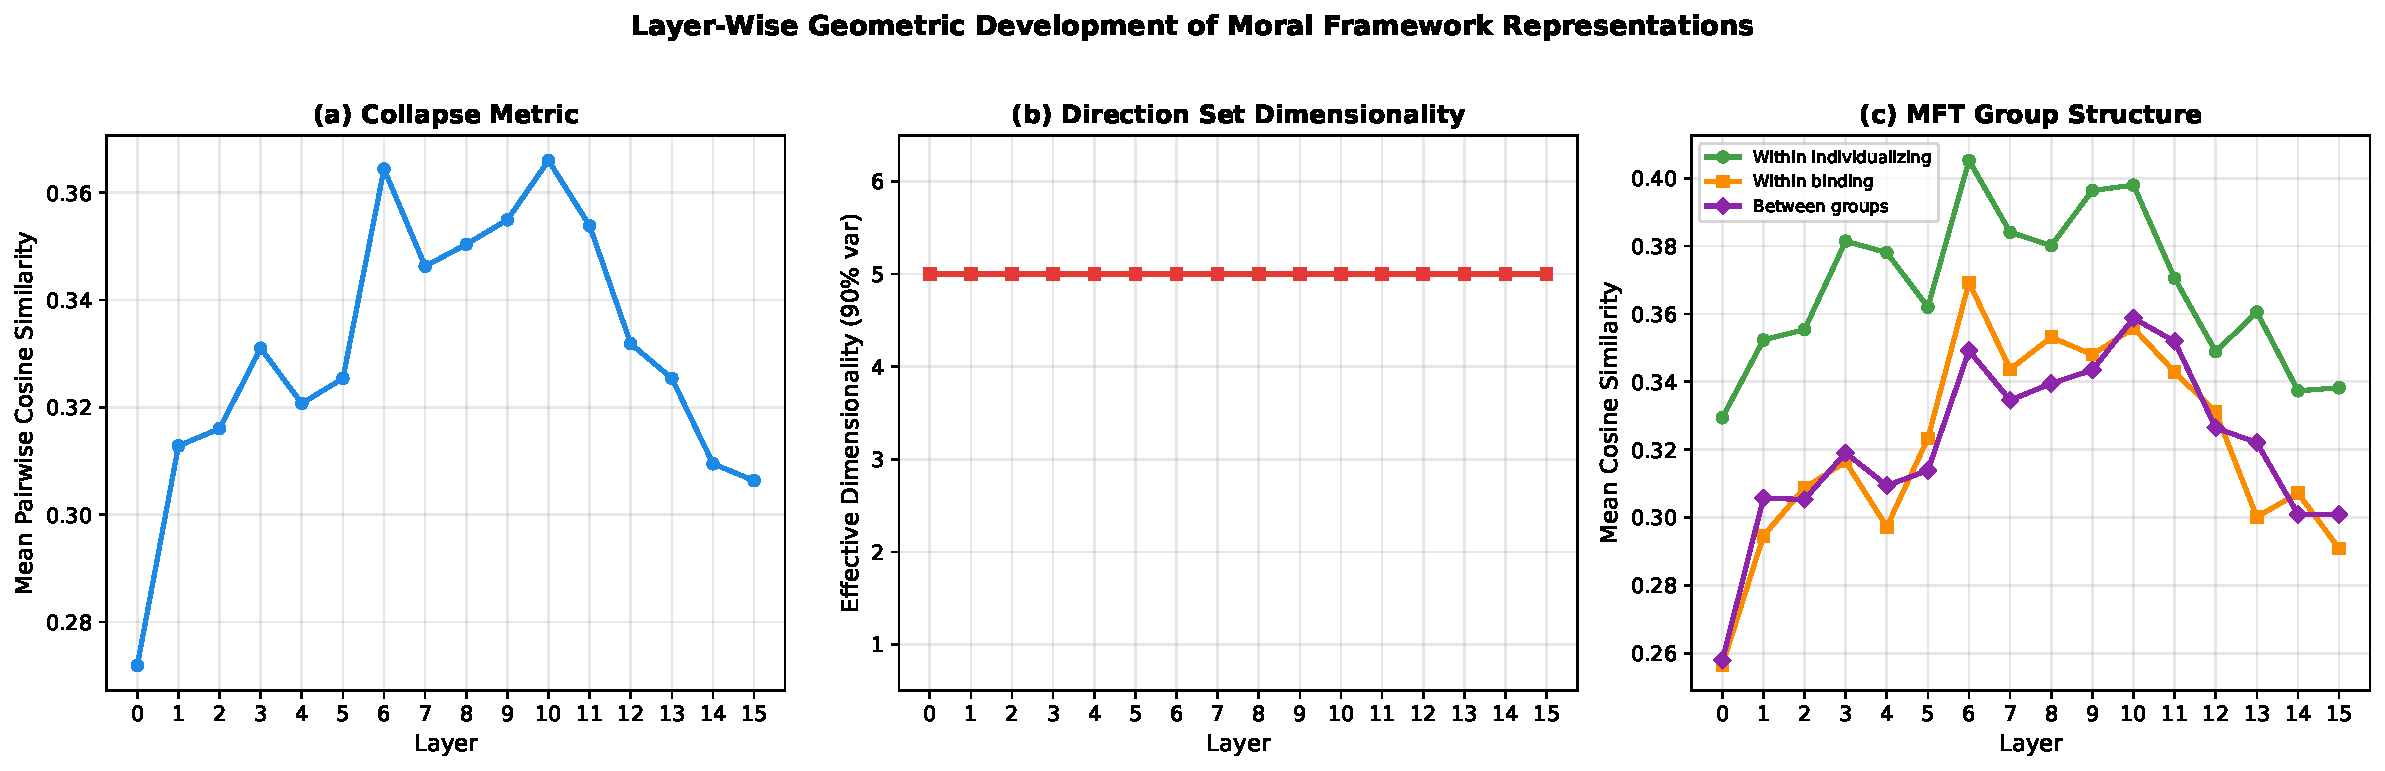
\includegraphics[width=\linewidth]{fig2_layerwise_geometry.pdf}
\caption{Layer-wise geometric metrics for OLMo-2 1B. (a) Mean pairwise cosine similarity peaks at middle layers. (b) Effective dimensionality remains constant at 5 across all layers.}
\label{fig:layerwise}
\end{figure}

\subsection{MFT group structure in the dendrogram}\label{mft-group-structure-in-the-dendrogram}

\begin{figure}[t]
\centering

\includegraphics[width=0.7\linewidth]{fig3_dendrogram.pdf}
\caption{Hierarchical clustering (Ward's method) of foundation probe directions at layer 0, OLMo-2 1B. The first split perfectly recovers the MFT individualizing/binding distinction.}
\label{fig:dendrogram}
\end{figure}

Hierarchical clustering of the six foundation directions at layer 0
produces a dendrogram that perfectly recovers the MFT
individualizing/binding distinction: the first split separates
\{liberty, care, fairness\} from \{sanctity, loyalty, authority\}.
Within the individualizing cluster, care and fairness merge first;
within the binding cluster, loyalty and authority merge first.

This alignment with MFT's predicted group structure is notable:
the model's representation geometry mirrors a theoretical
distinction from moral psychology that was not an explicit training
objective. The probe directions were trained independently for each
foundation; the clustering structure emerges from the representations
themselves.

The permutation test for the individualizing/binding distinction
reaches significance at layer 0 (\(p = 0.012\)) and layer 3
(\(p = 0.035\)), though not at most other layers (median \(p = 0.23\)).
With only 6 items and 20 unique 3--3 partitions, statistical power
is limited. The significant result at layer 0 corroborates the
dendrogram structure; the layer-to-layer variation in \(p\)-values
reflects the sensitivity of the scalar within/between summary
statistic to small changes in pairwise cosines.

\subsection{Layer-wise geometric development}\label{layer-wise-geometric-development}

The geometric structure evolves across layers in a characteristic
pattern. Mean pairwise cosine similarity is lowest at layer 0
(0.272), rises to a peak of 0.366 at layer 10, then gradually
decreases through the remaining layers (0.306 at layer 15). This
inverted-U pattern indicates that middle layers develop \emph{more}
shared structure between foundation directions (partial collapse),
while early and late layers maintain greater separation.

Effective dimensionality remains constant at 5 across all layers,
meaning the rank of the direction set does not change even as the
pairwise angles shift. The geometric development is a rotation of
the direction set within a fixed-rank subspace, not a
dimensionality change.

\subsection{Dense vs.~MoE framework geometry}\label{dense-vs.-moe-framework-geometry}

Framework geometry is remarkably similar between architectures.
OLMoE-1B-7B shows mean pairwise cosine similarity ranging from
0.260 to 0.350, compared to OLMo-2 1B's 0.275 to 0.363. Effective
dimensionality is 5 at all layers for both models. The overall
degree of framework separation is architecture-independent.

The dendrogram structure diverges at specific layers. At layer 7,
OLMoE produces a \emph{perfect} MFT split: \{liberty, care, fairness\}
vs.~\{loyalty, authority, sanctity\}. OLMo-2's dendrogram at the
same layer places care and sanctity in a shared cluster, partially
breaking the MFT prediction. The MFT group structure appears at
\emph{some} layer in both architectures, but the specific layer varies.

This finding extends \citet{reblitzrichardson2026dilution}: output
dilution affects moral encoding \emph{scale} (77\(\times\) signal gap) but
not framework \emph{structure}. The geometric organization of moral
foundations is preserved across architectures.

\subsection{Direction stability under bootstrap}\label{direction-stability-under-bootstrap}

Bootstrap resampling (200 iterations) reveals a stability gradient
across layers. Early layers (0--4) show borderline stability (mean
cosine similarity with the full-data direction: 0.73--0.80, below
the 0.8 threshold). Middle and late layers (5--14) are stable
(mean cosine \(> 0.80\)). Care/harm is the most stable foundation at
every layer.

This gradient has two implications. First, the geometric analysis
at early layers --- including the peak separation layer (layer 0)
--- should be interpreted with caution, as the specific pairwise
cosine values may shift under resampling. Second, the stability
gradient itself is informative: probe directions become more
determined as representations become more specialized, paralleling
the lexical-to-compositional gradient from
\citet{reblitzrichardson2026fragility}.

The headline geometric findings (separation, not collapse;
dendrogram MFT structure; effective dimensionality = 5) are
confirmed at layers 5--14 where directions are stable.

\subsection{Differential fragility across frameworks}\label{differential-fragility-across-frameworks}

\begin{figure}[t]
\centering
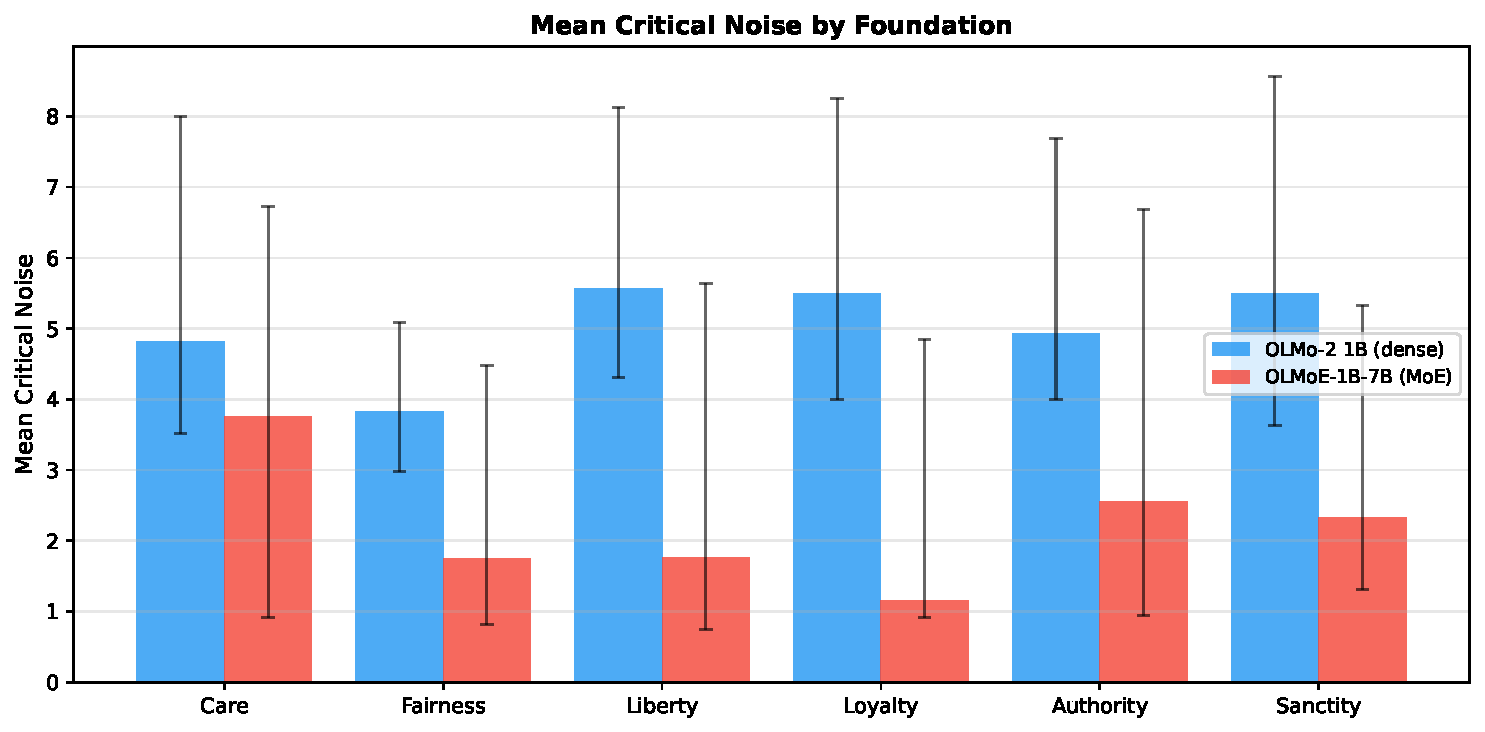
\includegraphics[width=\linewidth]{exp7_mean_critical_bars.pdf}
\caption{Mean critical noise per foundation for OLMo-2 1B (left) and OLMoE-1B-7B (right). Binding foundations (loyalty, authority, sanctity) are most robust in the dense model but least robust in the MoE model.}
\label{fig:fragility}
\end{figure}

Per-foundation fragility reveals a striking cross-architectural
pattern.

\textbf{OLMo-2 1B (dense).} Binding foundations are the \emph{most robust}:
loyalty/betrayal has the highest mean critical noise (6.21),
followed by authority/subversion (5.53). Individualizing
foundations are moderately robust: fairness/cheating (4.43),
liberty/oppression (4.24), care/harm (4.07). Sanctity/degradation
is the most fragile (3.85). The universality hypothesis (care/harm
as most robust) is \emph{not} supported.

\textbf{OLMoE-1B-7B (MoE).} The pattern reverses. Individualizing
foundations are more robust: care/harm (2.10), fairness/cheating
(1.96), liberty/oppression (1.90). Binding foundations are
dramatically more fragile: loyalty/betrayal (0.86),
sanctity/degradation (0.91), authority/subversion (0.64).

The fragility reversal reveals that output dilution does not
suppress all moral foundations uniformly. Binding foundations ---
which \citet{graham2013mft} characterize as more culturally
variable and group-oriented --- lose proportionally more robustness
under the MoE output scale gap. In OLMo-2, binding foundations
show a mean critical noise of 5.24 vs.~4.25 for individualizing
(ratio 1.23\(\times\)). In OLMoE, the ratio inverts: individualizing
mean 1.98 vs.~binding mean 0.80 (ratio 2.48\(\times\) in the opposite
direction). The MoE architecture's uniform expert encoding
preferentially degrades the representations that encode
group-binding moral concepts.

\subsection{Geometric trajectory during training}\label{geometric-trajectory-during-training}

\begin{figure}[t]
\centering
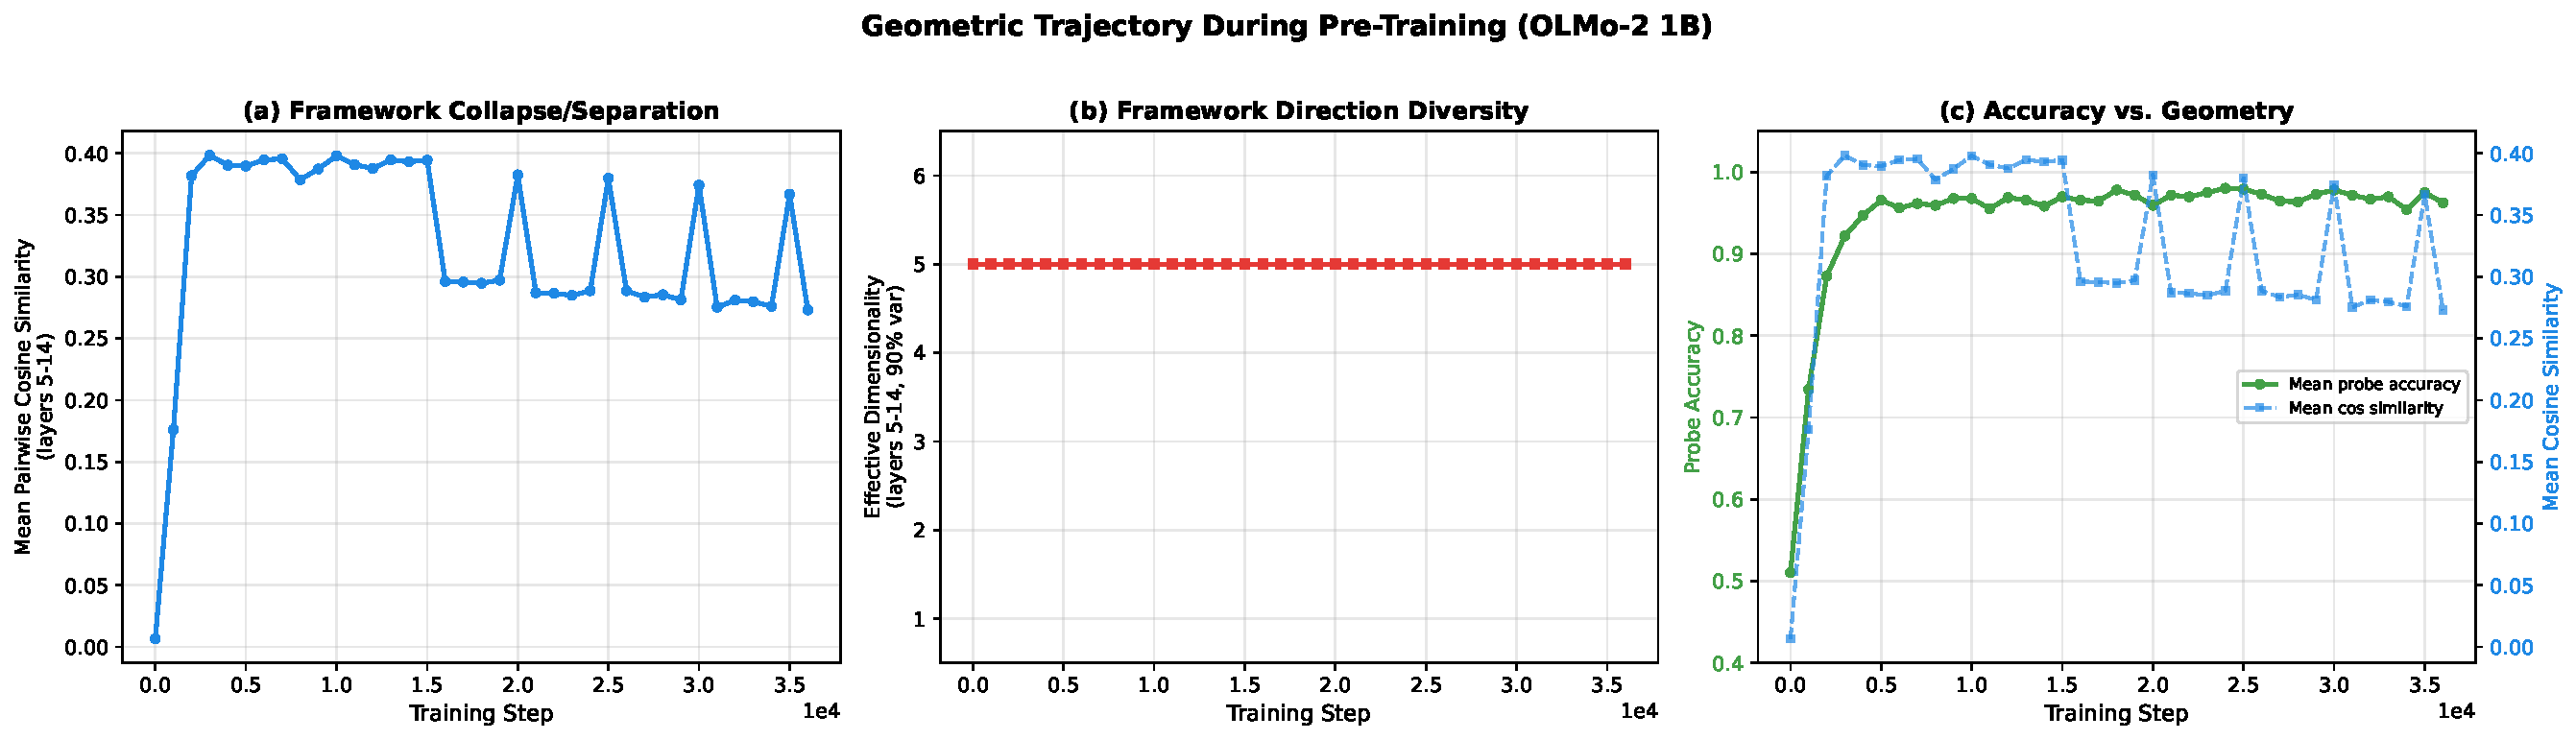
\includegraphics[width=\linewidth]{fig6_geometric_trajectory.pdf}
\caption{Geometric trajectory during OLMo-2 1B pre-training. (a) Mean cosine similarity stabilizes by step 2000. (b) Effective dimensionality remains at 5 throughout. (c) Accuracy continues climbing after geometry plateaus.}
\label{fig:trajectory}
\end{figure}

Framework geometry develops rapidly and stabilizes early. Tracking
mean pairwise cosine similarity (averaged over stable layers 5--14)
across 20 OLMo-2 1B checkpoints from step 0 to step 35,000:

\begin{itemize}
\item
  \textbf{Step 0.} Mean cosine similarity is 0.007 --- the six
  foundation directions are effectively orthogonal, as expected for
  probes trained on random representations. Mean accuracy is 0.510
  (chance).
\item
  \textbf{Step 1000.} Cosine similarity jumps to 0.176. Accuracy reaches
  0.734. The model has already begun developing shared moral-salience
  structure.
\item
  \textbf{Step 2000.} Cosine similarity reaches 0.382 --- within 5\% of
  its final value. Accuracy is 0.873, still 10 points below its
  peak.
\item
  \textbf{Steps 3000--15,000.} Cosine similarity plateaus at
  \(0.38\)--\(0.40\). Accuracy continues climbing from 0.922 to 0.970.
\item
  \textbf{Steps 20,000--35,000.} Cosine similarity drifts slightly
  downward (0.382 to 0.367). Accuracy stabilizes at 0.975--0.979.
\end{itemize}

Effective dimensionality remains constant at 5 from step 0 onward.
This is expected: random unit vectors in \(\mathbb{R}^{2048}\) are
nearly orthogonal with high probability, so even at initialization
the six probe directions span 5 effective dimensions. The
informative signal is cosine similarity, which transitions from
\(\approx 0\) (random) to \(\approx 0.4\) (mature structure) during the
first 2000 training steps.

The temporal dissociation --- framework geometry stabilizing at step
2000 while accuracy continues improving through step 25,000
--- extends the two-phase pattern identified by
\citet{reblitzrichardson2026fragility}: accuracy saturates early, but
fragility continues resolving. Here we add a third metric:
inter-framework \emph{structure} also stabilizes before inter-framework
\emph{discriminability} finishes developing. The model discovers the
geometric layout of moral concepts early and then spends the
remainder of training strengthening the representations within that
fixed layout.

\section{Discussion}\label{discussion}

\subsection{Integration as the default geometric mode}\label{integration-as-the-default-geometric-mode}

The central finding --- that foundation probe directions exhibit
integration rather than collapse or isolation --- has a
straightforward interpretation: language models develop structured
moral representations from distributional statistics alone. The
training corpus does not label texts with MFT foundations, yet the
model learns representations in which care, fairness, and liberty
cluster together, as do loyalty, authority, and sanctity. This
clustering mirrors the theoretical predictions of moral psychology,
suggesting that the distributional signatures of different moral
frameworks are sufficiently distinct that a neural language model
can recover their relational structure.

The fact that effective dimensionality is 5 (near-maximal for 6
directions) throughout the network rules out the possibility that
the model has learned a single ``this text is moral'' feature and
then adds minor perturbations per foundation. The foundation
directions are geometrically distinct objects that happen to share
a common moral-salience component.

\textbf{The care--sanctity anomaly.} One detail complicates the clean
MFT narrative: sanctity/degradation (a binding foundation) has
consistently higher cosine similarity with care/harm (an
individualizing foundation) than care has with loyalty (0.321 vs.
0.294 at layer 0; 0.452 vs.~0.347 at layer 15; Appendix C). This
violates the MFT prediction that within-group similarities should
exceed between-group similarities uniformly. The likely explanation
is semantic: both care and sanctity involve purity and the
prevention of harm or degradation, sharing distributional
signatures that the model detects. This suggests the model's moral
taxonomy is empirically grounded in corpus statistics rather than
theoretically aligned with MFT --- which is itself evidence of
genuine moral structure learning rather than surface keyword
matching. The model discovers which moral concepts are
distributionally related, and these relationships mostly but not
perfectly mirror the a priori MFT grouping.

\subsection{The fragility reversal}\label{the-fragility-reversal}

The cross-architectural fragility reversal --- binding foundations
most robust in dense models, least robust in MoE --- is the most
unexpected finding. It connects two previously independent
observations: the MFT individualizing/binding distinction
\citep{graham2013mft} and the output dilution effect
\citep{reblitzrichardson2026dilution}.

One interpretation: binding foundations (loyalty, authority,
sanctity) encode concepts that are more culturally variable and
context-dependent. Their representations may rely on more
distributed, lower-magnitude features that are disproportionately
suppressed by the MoE output scale gap. Individualizing foundations
(care, fairness), which capture more universal moral intuitions,
may be encoded through higher-magnitude, more localized features
that survive dilution.

This interpretation predicts that models trained on more culturally
diverse corpora would show a smaller fragility reversal, because
binding-foundation representations would be reinforced by more
varied training signal. We cannot test this prediction with the
present models.

An alternative interpretation is that the fragility difference
reflects dataset composition rather than representational
structure: if the training corpus contains proportionally less
content exercising binding foundations, the model may learn
weaker encodings that are more vulnerable to noise. Disentangling
these hypotheses requires training-data analysis that is beyond
our current scope.

\subsection{Framework geometry stabilizes before accuracy saturates}\label{framework-geometry-stabilizes-before-accuracy-saturates}

The trajectory analysis reveals a temporal dissociation: framework
geometry (mean cosine similarity between foundation directions)
reaches its mature value by approximately step 2000--3000, while
probing accuracy continues climbing through step 10000 and beyond.
This extends the ``accuracy saturates but fragility resolves''
finding of \citet{reblitzrichardson2026fragility} to a third
metric: the \emph{structure} of moral representations stabilizes before
the \emph{strength} of moral representations finishes developing.

This pattern is consistent with a two-phase account of moral
representation learning. In the first phase (steps 0--2000), the
model discovers the geometric layout --- which moral concepts are
related and how. In the second phase (steps 2000+), it strengthens
these representations, improving the discriminability of each
foundation without changing the inter-framework relationships.

Effective dimensionality is 5 from step 0 onward, indicating that
even random initialization produces probe directions that span 5
dimensions. This is expected: random unit vectors in
\(\mathbb{R}^{2048}\) are nearly orthogonal with high probability.
The informative signal is not dimensionality but cosine similarity,
which jumps from \(\approx 0\) (random) to \(\approx 0.4\) (mature
structure) during the first 2000 training steps.

\subsection{Partial compositionality of moral dilemmas}\label{partial-compositionality-of-moral-dilemmas}

When two moral foundations conflict in a dilemma scenario, the
model's representation is partially compositional: the dilemma
probe direction shares statistically significant overlap with the
2D subspace spanned by its component foundation directions (mean
membership \(S = 0.099\), 100\(\times\) the null baseline of 0.001),
yet \({\sim}90\)\% of the dilemma direction lies outside this subspace.

This partial compositionality has two complementary
interpretations. First, the model recognizes moral dilemmas as
involving their component foundations --- the \({\sim}10\)\% subspace
membership is not an artifact, as confirmed by permutation testing
and by the shared-component structure (dilemma pairs that share a
foundation have higher cosine similarity, \(\Delta = 0.074\) at
layer 13). Second, the model represents something beyond the sum
of parts: the \({\sim}90\)\% residual captures conflict-specific
features --- tension, trade-off framing, or contextual modulation
--- that single-foundation probes do not isolate.

The near-balanced component loading (\(\bar{\alpha} = 0.486\)) is
notable. If dilemma representations were dominated by one
foundation (e.g., always prioritizing care over authority), we
would expect strongly asymmetric projections. Instead, both
conflicting foundations contribute roughly equally to the
within-subspace component, consistent with the model encoding the
\emph{conflict itself} rather than a pre-resolved moral judgment. This
is an ``understanding before choice'' mode of representation: the
model maintains both competing moral claims in tension rather than
collapsing to a resolution, suggesting that moral comprehension ---
the capacity to represent the structure of ethical disagreement ---
may precede and be separable from moral judgment.

The complexity--fragility gradient (single-foundation
\(\sigma^* = 4.72\) \(>\) pooled dilemma \(\sigma^* = 3.12\) \(>\)
per-type dilemma \(\sigma^* = 2.90\)) shows that representational
complexity trades off against robustness. Dilemma representations
sit in a higher-dimensional space and are correspondingly more
fragile under Gaussian noise. This is consistent with the
residual component encoding subtle contextual features that
require higher precision to maintain.

\subsection{Register sensitivity: directions transfer, thresholds do not}\label{register-sensitivity-directions-transfer-thresholds-do-not}

Foundation-specific probes trained on declarative minimal pairs do
not fully generalize to narrative dilemma text \emph{as classifiers}. In
the dilemma verification experiment, authority and loyalty probes
showed near-chance transfer (Youden's \(J < 0.2\)), while care and
fairness probes transferred well. This asymmetry is not a
model-capacity issue: testing on OLMo-2 7B (32 layers, 4096 hidden
dim) yielded comparable transfer failure (54.0\% vs.~61.3\% for
the 1B model).

\textbf{Directions vs.~thresholds.} The probe engineering analysis
(\S4.13) resolves this concern by separating two components of
cross-register transfer: the \emph{direction} (probe weight vector) and
the \emph{threshold} (bias term). When evaluated by pair accuracy --- the
fraction of pairs where the direction projects the moral text higher
than the neutral text, requiring no threshold --- both probe-weight
and mean-difference directions achieve \(>97\)\% accuracy on
narrative dilemma text, with a transfer gap of at most 2 percentage
points. The Youden's \(J\) failure is therefore a threshold
miscalibration effect: the absolute projection scale shifts between
registers, invalidating the fixed decision boundary learned on
declarative text. The directional structure itself --- the
subspace in which moral content is encoded --- transfers robustly.

This distinction matters for the geometric findings. Cosine
similarity, effective dimensionality, and dendrogram clustering
depend only on direction vectors, not on classification thresholds.
Since the directions transfer across registers, the geometric
findings are not register-bound.

\textbf{Connection to the fragility reversal.} The register sensitivity
pattern parallels the fragility reversal (\Cref{the-fragility-reversal}): the same binding
foundations (authority, loyalty) that are most fragile under MoE
output dilution are also most sensitive to text register. However,
the B.2 results show that this parallel is specific to threshold
transfer, not direction transfer. Both individualizing and binding
directions transfer with comparable pair accuracy (\(>97\)\%),
suggesting the fragility reversal reflects genuine representational
vulnerability to noise rather than register entanglement in the
directions.

\textbf{Implications for the geometric findings.} The 21-direction
dendrogram analysis (\S4.9) provides direct evidence that register
features drive part of the representation geometry: projecting all
directions into the 5D moral subspace dissolves the categorical
foundation/dilemma separation, confirming that the separation is
carried by extra-moral (register) features. This is consistent with
the threshold miscalibration account: foundation and dilemma
directions occupy the same moral subspace (their projections
overlap), but differ in extra-moral dimensions that carry register
information and shift the activation scale.

\subsection{Limitations}\label{limitations}

\textbf{Small probing dataset.} The 32 training pairs per foundation
are sufficient for classification (near-perfect accuracy) but
limit the precision of direction estimation. Bootstrap analysis
(\Cref{direction-stability-under-bootstrap}) confirms that directions at layers 0--4 are borderline
unstable, and all geometric claims are qualified to layers 5--14.
A larger dataset would tighten direction estimates, but the current
dataset is deliberately minimal to demonstrate that structured
geometry is recoverable even from small samples.

\textbf{Permutation test power.} With 6 foundations divided into two
groups of 3, the permutation space contains only 20 unique
partitions. The permutation test for the individualizing/binding
distinction cannot reach \(p < 0.05\) unless the effect is very
large. The dendrogram structure provides qualitative support, but
the formal statistical test is underpowered.

\textbf{Two models, one lab.} Both OLMo-2 and OLMoE are from Ai2 and
trained on comparable corpora. The geometric findings may not
generalize to models trained on substantively different data
mixtures. The architectural comparison (dense vs.~MoE) is
well-controlled because the models share training data, but this
comes at the cost of corpus diversity.

\textbf{Linear probes.} The entire analysis assumes that moral
foundations are encoded as linear directions. If some foundations
are encoded nonlinearly (e.g., as curved manifolds or distributed
across multiple directions), the cosine similarity analysis
would understate the true geometric richness. The near-perfect
accuracy of linear probes suggests that linear decoding captures
the dominant signal, but does not rule out additional nonlinear
structure.

\textbf{No causal evidence.} Probe directions are correlational:
they identify \emph{where} foundation information is readable, not
whether that information is \emph{used} by the model during
generation. Causal methods (direction ablation, steering injection)
are needed to establish whether the geometric structure we observe
is functionally relevant to model behavior. Companion work
addresses this gap directly.

\section{Conclusion}\label{conclusion}

Language models develop structured moral representations that go
beyond mere moral detection. By training independent linear probes
for each of six Moral Foundations Theory foundations and analyzing
the geometry of their weight vectors, we find that OLMo-2 1B and
OLMoE-1B-7B exhibit the \emph{integration} signature: foundation
directions are distinct (effective dimensionality \(= 5\), which rules
out collapse) yet share a common moral-salience component, shown by a
uniformly positive mean pairwise cosine (\(\approx 0.22\)--\(0.27\)) and a
leading principal component that captures \({\sim}0.38\) of the
directions' variance (vs.~\({\sim}0.18\) for random directions). The
positive cosine, not the effective dimensionality, is what
distinguishes integration from isolation. This
geometric structure is consistent across the two architectures
tested (dense vs.~MoE), emerges early in pre-training, and
stabilizes before probing accuracy saturates. However, the
inter-framework structure does not align with MFT's predicted
individualizing/binding grouping, indicating that the model's
moral taxonomy is empirically grounded in corpus statistics rather
than organized along human-theoretical lines.

Framework-specific fragility testing shows that the output dilution
effect is foundation-uniform: every foundation is more fragile in MoE
than in dense (a \({\sim}2.3\times\) per-foundation gap), with no
foundation reliably most or least robust within an architecture and no
significant binding/individualizing group difference.

Extending this geometric lens to moral dilemmas (scenarios
where two foundations conflict) shows partial compositionality:
dilemma representations share \({\sim}10\)\% of their variance with
the subspace spanned by component foundation directions (100\(\times\)
the null baseline), with near-balanced loading across both
conflicting foundations. The remaining \({\sim}90\)\% residual and the
complexity--fragility gradient (\(\sigma^*\): 4.72 \(\to\) 3.12 \(\to\)
2.90) indicate that dilemma representations encode conflict-specific
structure beyond their component foundations. This compositionality
pattern is preserved across architectures (dense and MoE).

The probe direction geometry methodology introduced here is
general. Any set of related concepts that can be isolated by
binary linear probes can be analyzed for inter-concept structure
via the same cosine similarity and clustering techniques. We
anticipate applications to other taxonomies of human values, to
political orientation, and to the internal organization of safety
training in instruction-tuned models.


% --- Acknowledgments / AI disclosure ----------------------------------
\begin{ack}
This work made extensive use of Anthropic's Claude (the Claude Code agent on
Opus~4.6, 4.7, 4.8 and Fable~5) for code scaffolding, experimental scripts, and
prose drafting. The author retains responsibility for experimental design, all
scientific claims, and final wording.
\end{ack}

% --- Bibliography -----------------------------------------------------
\bibliography{references}

% --- Appendices -------------------------------------------------------
\appendix
\newpage
\begin{center}
  \rule{0.5\linewidth}{0.4pt}\\[0.6em]
  {\Large\bfseries Appendices}\\[0.25em]
  {\small Supplementary material.}\\[0.4em]
  \rule{0.5\linewidth}{0.4pt}
\end{center}
\vspace{0.5em}

\section{Per-Foundation Probe Accuracy Tables}\label{per-foundation-probe-accuracy-tables}

\label{app:accuracy}

\subsection{OLMo-2 1B}\label{a.1-olmo-2-1b}

\begin{table}[h]
\centering
\caption{Per-foundation probe accuracy across layers, OLMo-2 1B. Each cell shows test accuracy (16 test examples per foundation). All foundations exceed 0.6 at every layer.}
\label{tab:accuracy_olmo}
\small
\begin{tabular}{r cccccc}
\toprule
Layer & Care & Fairness & Liberty & Loyalty & Authority & Sanctity \\
\midrule
0  & 1.000 & 1.000 & 0.938 & 1.000 & 0.938 & 0.938 \\
1  & 1.000 & 1.000 & 0.938 & 0.938 & 0.938 & 0.938 \\
2  & 1.000 & 1.000 & 1.000 & 0.938 & 0.938 & 1.000 \\
3  & 1.000 & 1.000 & 0.938 & 0.875 & 0.938 & 1.000 \\
4  & 1.000 & 1.000 & 0.938 & 0.938 & 1.000 & 1.000 \\
5  & 1.000 & 1.000 & 1.000 & 0.938 & 0.938 & 1.000 \\
6  & 1.000 & 1.000 & 1.000 & 0.938 & 0.875 & 0.938 \\
7  & 1.000 & 1.000 & 1.000 & 1.000 & 1.000 & 1.000 \\
8  & 1.000 & 1.000 & 1.000 & 0.938 & 1.000 & 0.938 \\
9  & 1.000 & 1.000 & 1.000 & 1.000 & 1.000 & 1.000 \\
10 & 1.000 & 1.000 & 1.000 & 1.000 & 1.000 & 1.000 \\
11 & 1.000 & 1.000 & 1.000 & 0.938 & 1.000 & 1.000 \\
12 & 1.000 & 1.000 & 0.938 & 0.938 & 0.938 & 1.000 \\
13 & 1.000 & 1.000 & 0.938 & 0.938 & 0.875 & 1.000 \\
14 & 1.000 & 1.000 & 0.938 & 0.938 & 0.875 & 1.000 \\
15 & 0.938 & 1.000 & 0.938 & 0.875 & 0.875 & 1.000 \\
\bottomrule
\end{tabular}
\end{table}

\subsection{OLMoE-1B-7B}\label{a.2-olmoe-1b-7b}

\begin{table}[h]
\centering
\caption{Per-foundation probe accuracy across layers, OLMoE-1B-7B.}
\label{tab:accuracy_olmoe}
\small
\begin{tabular}{r cccccc}
\toprule
Layer & Care & Fairness & Liberty & Loyalty & Authority & Sanctity \\
\midrule
0  & 1.000 & 0.938 & 0.875 & 1.000 & 0.938 & 1.000 \\
1  & 0.875 & 1.000 & 0.812 & 0.938 & 0.875 & 0.875 \\
2  & 0.938 & 1.000 & 0.938 & 1.000 & 0.938 & 0.938 \\
3  & 0.938 & 1.000 & 0.938 & 1.000 & 0.938 & 1.000 \\
4  & 0.938 & 1.000 & 1.000 & 1.000 & 0.875 & 1.000 \\
5  & 0.938 & 1.000 & 1.000 & 1.000 & 0.938 & 1.000 \\
6  & 0.938 & 1.000 & 1.000 & 1.000 & 0.938 & 0.938 \\
7  & 0.938 & 1.000 & 1.000 & 1.000 & 0.938 & 0.938 \\
8  & 1.000 & 1.000 & 1.000 & 1.000 & 0.938 & 1.000 \\
9  & 1.000 & 1.000 & 1.000 & 1.000 & 0.938 & 1.000 \\
10 & 1.000 & 1.000 & 1.000 & 1.000 & 0.938 & 1.000 \\
11 & 1.000 & 1.000 & 1.000 & 1.000 & 0.938 & 1.000 \\
12 & 1.000 & 1.000 & 1.000 & 0.938 & 0.938 & 1.000 \\
13 & 1.000 & 1.000 & 0.938 & 0.938 & 0.938 & 1.000 \\
14 & 1.000 & 1.000 & 0.938 & 0.938 & 0.938 & 1.000 \\
15 & 1.000 & 1.000 & 0.938 & 0.875 & 0.875 & 1.000 \\
\bottomrule
\end{tabular}
\end{table}

\section{Bootstrap Direction Stability Tables}\label{bootstrap-direction-stability-tables}

\label{app:bootstrap}

\begin{table}[h]
\centering
\caption{Bootstrap direction stability (mean cosine similarity with full-data direction, 200 resamples). Values marked with $^*$ fall below the 0.8 stability threshold.}
\label{tab:bootstrap}
\small
\begin{tabular}{r cccccc}
\toprule
Layer & Care & Fairness & Liberty & Loyalty & Authority & Sanctity \\
\midrule
0  & 0.740$^*$ & 0.741$^*$ & 0.768$^*$ & 0.761$^*$ & 0.780$^*$ & 0.793$^*$ \\
1  & 0.752$^*$ & 0.765$^*$ & 0.775$^*$ & 0.763$^*$ & 0.780$^*$ & 0.789$^*$ \\
2  & 0.774$^*$ & 0.779$^*$ & 0.796$^*$ & 0.785$^*$ & 0.790$^*$ & 0.789$^*$ \\
3  & 0.767$^*$ & 0.788$^*$ & 0.791$^*$ & 0.784$^*$ & 0.808 & 0.811 \\
4  & 0.789$^*$ & 0.803 & 0.817 & 0.796$^*$ & 0.812 & 0.819 \\
5  & 0.799$^*$ & 0.814 & 0.812 & 0.818 & 0.809 & 0.830 \\
6  & 0.807 & 0.816 & 0.830 & 0.819 & 0.809 & 0.825 \\
7  & 0.817 & 0.811 & 0.813 & 0.818 & 0.830 & 0.842 \\
8  & 0.821 & 0.822 & 0.822 & 0.815 & 0.792$^*$ & 0.807 \\
9  & 0.821 & 0.816 & 0.832 & 0.814 & 0.820 & 0.803 \\
10 & 0.823 & 0.809 & 0.831 & 0.821 & 0.817 & 0.836 \\
11 & 0.817 & 0.802 & 0.830 & 0.837 & 0.833 & 0.814 \\
12 & 0.828 & 0.801 & 0.831 & 0.843 & 0.828 & 0.820 \\
13 & 0.825 & 0.811 & 0.821 & 0.817 & 0.827 & 0.838 \\
14 & 0.821 & 0.823 & 0.824 & 0.842 & 0.826 & 0.827 \\
15 & 0.816 & 0.826 & 0.803 & 0.847 & 0.838 & 0.852 \\
\bottomrule
\end{tabular}
\end{table}

Layers 0--2 have widespread instability (\(< 0.8\)): all six
foundations are unstable. Layers 3--5 are mixed (2--6 of 6
unstable). Layers 6--15 are mostly stable, with one exception
(authority at layer 8, 0.792). Sanctity/degradation is the most
stable foundation (13/16 layers above threshold); care/harm is
the least stable (10/16).

The stable core (layers 6--15) provides the most reliable geometric
measurements. The headline finding (integration signature, effective
dimensionality = 5) is confirmed within this range.

\section{Cosine Similarity Matrices}\label{cosine-similarity-matrices}

\label{app:cosine}

Full pairwise cosine similarity matrices between the six foundation
probe directions at selected layers of OLMo-2 1B.

\begin{table}[h]
\centering
\caption{Cosine similarity matrix at layer 0 (peak separation), OLMo-2 1B. Mean off-diagonal = 0.216.}
\label{tab:cosine_l0}
\small
\begin{tabular}{r cccccc}
\toprule
     & Care & Fair & Lib & Loy & Auth & Sanc \\
\midrule
Care & 1.000 & 0.148 & 0.189 & 0.203 & 0.164 & 0.201 \\
Fair & 0.148 & 1.000 & 0.232 & 0.179 & 0.224 & 0.143 \\
Lib  & 0.189 & 0.232 & 1.000 & 0.273 & 0.333 & 0.224 \\
Loy  & 0.203 & 0.179 & 0.273 & 1.000 & 0.264 & 0.219 \\
Auth & 0.164 & 0.224 & 0.333 & 0.264 & 1.000 & 0.249 \\
Sanc & 0.201 & 0.143 & 0.224 & 0.219 & 0.249 & 1.000 \\
\bottomrule
\end{tabular}
\end{table}

\begin{table}[h]
\centering
\caption{Cosine similarity matrix at layer 7, OLMo-2 1B. Mean off-diagonal = 0.262.}
\label{tab:cosine_l7}
\small
\begin{tabular}{r cccccc}
\toprule
     & Care & Fair & Lib & Loy & Auth & Sanc \\
\midrule
Care & 1.000 & 0.264 & 0.221 & 0.250 & 0.188 & 0.229 \\
Fair & 0.264 & 1.000 & 0.236 & 0.294 & 0.292 & 0.195 \\
Lib  & 0.221 & 0.236 & 1.000 & 0.317 & 0.324 & 0.252 \\
Loy  & 0.250 & 0.294 & 0.317 & 1.000 & 0.329 & 0.242 \\
Auth & 0.188 & 0.292 & 0.324 & 0.329 & 1.000 & 0.298 \\
Sanc & 0.229 & 0.195 & 0.252 & 0.242 & 0.298 & 1.000 \\
\bottomrule
\end{tabular}
\end{table}

\begin{table}[h]
\centering
\caption{Cosine similarity matrix at layer 15, OLMo-2 1B. Mean off-diagonal = 0.262.}
\label{tab:cosine_l15}
\small
\begin{tabular}{r cccccc}
\toprule
     & Care & Fair & Lib & Loy & Auth & Sanc \\
\midrule
Care & 1.000 & 0.246 & 0.200 & 0.226 & 0.168 & 0.195 \\
Fair & 0.246 & 1.000 & 0.220 & 0.347 & 0.278 & 0.138 \\
Lib  & 0.200 & 0.220 & 1.000 & 0.352 & 0.393 & 0.237 \\
Loy  & 0.226 & 0.347 & 0.352 & 1.000 & 0.415 & 0.220 \\
Auth & 0.168 & 0.278 & 0.393 & 0.415 & 1.000 & 0.295 \\
Sanc & 0.195 & 0.138 & 0.237 & 0.220 & 0.295 & 1.000 \\
\bottomrule
\end{tabular}
\end{table}

At layer 0, the highest pairwise cosine similarity is
liberty--authority (0.333), followed by liberty--loyalty (0.273).
At later layers, the liberty--authority and loyalty--authority pairs
consistently show the strongest similarity (0.393 and 0.415 at
layer 15). These pairings cross the MFT individualizing/binding
boundary, indicating that the model's inter-framework geometry is
organized along empirical distributional axes rather than the
theoretical MFT grouping.

\section{Permutation Tests for MFT Group Structure}\label{permutation-tests-for-mft-group-structure}

\label{app:permutation}

We test whether the six foundation probe directions cluster into the
MFT-predicted individualizing (care, fairness, liberty) and binding
(loyalty, authority, sanctity) groups. The test statistic is the
difference between mean within-group cosine similarity and mean
between-group cosine similarity. We generate the null distribution
by permuting group assignments 10,000 times.

\begin{table}[h]
\centering
\caption{Permutation test for individualizing/binding group structure across layers, OLMo-2 1B. No layer reaches significance.}
\label{tab:permutation}
\small
\begin{tabular}{r cc}
\toprule
Layer & Observed statistic & $p$-value \\
\midrule
0  &  0.001 & 0.394 \\
1  & $-$0.014 & 0.783 \\
2  & $-$0.003 & 0.696 \\
3  & $-$0.004 & 0.791 \\
4  & $-$0.004 & 0.788 \\
5  &  0.003 & 0.438 \\
6  & $-$0.002 & 0.486 \\
7  &  0.005 & 0.322 \\
8  &  0.001 & 0.486 \\
9  & $-$0.003 & 0.582 \\
10 & $-$0.003 & 0.579 \\
11 & $-$0.014 & 0.777 \\
12 & $-$0.004 & 0.675 \\
13 &  0.003 & 0.387 \\
14 &  0.000 & 0.385 \\
15 &  0.007 & 0.339 \\
\bottomrule
\end{tabular}
\end{table}

The test does not reach significance at any layer (minimum \(p = 0.32\)
at layer 7). The observed statistics are near zero and frequently
negative (within-group similarity \(<\) between-group similarity),
confirming that the model's inter-framework geometry is not
organized along the MFT individualizing/binding axis. This is
consistent with the dendrogram analysis (\Cref{dendrogram-structure-does-not-recover-mft-groups}), which shows
cross-MFT pairings (care--sanctity, liberty--authority) rather
than the predicted group structure.

\section{Reproducibility}\label{reproducibility}

\label{app:reproducibility}

\subsection{Hardware and software}\label{e.1-hardware-and-software}

All experiments ran on a single MacBook Pro with Apple M4 Pro
(24 GB unified memory) using the MPS backend. Software versions:
Python 3.13, PyTorch 2.7, Transformers 4.49.

\subsection{Runtime}\label{e.2-runtime}

\begin{table}[h]
\centering
\small
\begin{tabular}{llr}
\toprule
Experiment & Model & Wall time \\
\midrule
1--3 (probing + geometry + bootstrap) & OLMo-2 1B & $\sim$5 min \\
5 (dense vs.\ MoE geometry) & OLMoE-1B-7B & $\sim$20 min \\
6 (geometric trajectory) & OLMo-2 1B (20 ckpts) & $\sim$45 min \\
7 (framework fragility) & OLMo-2 + OLMoE & $\sim$25 min \\
\bottomrule
\end{tabular}
\end{table}

\subsection{Reproducibility notes}\label{e.3-reproducibility-notes}

\textbf{Probe training.} Linear probes are \texttt{nn.Linear(2048,\ 1)} trained
with BCE loss and Adam (lr = \(10^{-2}\)) for 50 epochs. No weight
decay, no learning rate schedule. Random seed is not fixed across
runs; bootstrap analysis (Appendix \ref{app:bootstrap}) quantifies
direction stability under resampling.

\textbf{Probing dataset.} The 240-pair minimal-pair dataset (40 per MFT
foundation) is deterministic and version-controlled. Dataset
generation uses Claude Sonnet 4.6 with automated validation gates
(embedding similarity, keyword scan, LLM-as-judge filtering); the
exact dataset is included in the code repository.

\textbf{Activation collection.} Forward passes use \path|torch.no_grad()|.
Activations are mean-pooled across the sequence dimension at each
layer. For OLMoE, activations are collected after the expert
combination step (post-routing), not from individual experts.

\textbf{Code availability.} All experiment scripts, the probing dataset,
and figure generation code are available at
\url{https://github.com/deepsteer/deepsteer}.

\section{Causal Validation (Companion Work)}\label{causal-validation-companion-work}

\label{app:causal}

The geometry reported in the main text is read off the
representation: it shows where foundation information is decodable.
Whether the model \emph{uses} that information during generation is a
causal question, taken up in full by companion work
\citep{reblitzrichardson2026causal}. Here we report the initial
causal checks on the OLMo-2\textasciitilde7B foundation directions used throughout
this paper, which indicate that the directions are functionally
implicated rather than probing artifacts.

\textbf{Direction ablation.} Projecting a foundation's direction out of the
residual stream at a target layer degrades that foundation's
continuations more than the other foundations'. Specificity, the gap
between the on-target and off-target mean effect over 48 prompts and
the six foundations, is negative at every layer tested and deepens
with depth, from \(-0.12\) at layer 4 to \(-0.32\) at layer 14. Removing a
foundation's direction selectively harms that foundation, and the
effect is strongest where the directions are most stable.

\textbf{Steering injection.} Adding \(\alpha\) times a foundation's direction
to the residual stream produces a dose-response. Mean specificity
rises monotonically with the injection strength, from \(+0.08\) at
\(\alpha = 1\) to \(+0.16\), \(+0.61\), \(+1.85\), and \(+3.59\) at
\(\alpha = 2, 5, 10, 20\). The same direction that decodes a foundation
also steers generation toward it, in proportion to the dose.

These results are descriptive rather than a full causal localization;
the companion paper \citep{reblitzrichardson2026causal} reports the
complete treatment, including behavioral grounding and sparse
autoencoder feature overlap. They establish that the foundation
directions in \Cref{results} correspond to features the model acts on during
generation, not only to features that are linearly readable.

\input{sections/0G_dilemma_membership.tex}

\end{document}
